\documentclass[tikz,border=10pt]{standalone}
% Scale s = 0.01214 cm/px, centred on ink bbox centre (403.5, 314.5) px, y flipped
\begin{document}
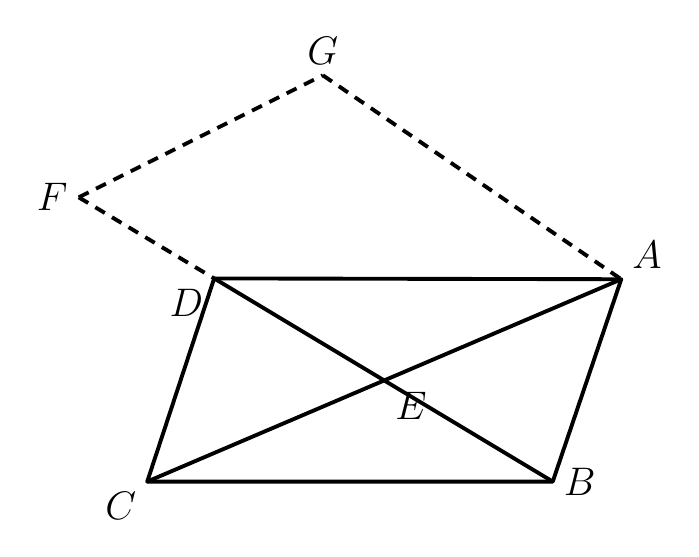
\begin{tikzpicture}[line width=1.4pt, line join=round]
  % Named coordinates (cm)
  \coordinate (A) at (3.45,-0.18);
  \coordinate (B) at (2.58,-2.75);
  \coordinate (C) at (-2.57,-2.75);
  \coordinate (D) at (-1.72,-0.17);
  \coordinate (E) at (0.44,-1.47);
  \coordinate (F) at (-3.44,0.86);
  \coordinate (G) at (-0.34,2.41);

  % Solid parallelogram ABCD and its diagonals
  \draw (A) -- (B) -- (C) -- (D) -- cycle;
  \draw (A) -- (C);
  \draw (B) -- (D);

  % Auxiliary edges GA, FG, FD: dashed, on 4pt off 3pt
  \draw[dash pattern=on 4pt off 3pt] (G) -- (A);
  \draw[dash pattern=on 4pt off 3pt] (F) -- (G);
  \draw[dash pattern=on 4pt off 3pt] (F) -- (D);

  % Labels
  \node[above right, font=\fontsize{15}{18}\selectfont] at (A) {$A$};
  \node[right, font=\fontsize{15}{18}\selectfont] at (B) {$B$};
  \node[below left, font=\fontsize{15}{18}\selectfont] at (C) {$C$};
  \node[below left, font=\fontsize{15}{18}\selectfont] at (D) {$D$};
  \node[below right, font=\fontsize{15}{18}\selectfont] at (E) {$E$};
  \node[left, font=\fontsize{15}{18}\selectfont] at (F) {$F$};
  \node[above, font=\fontsize{15}{18}\selectfont] at (G) {$G$};
\end{tikzpicture}
\end{document}